
\begin{figure}
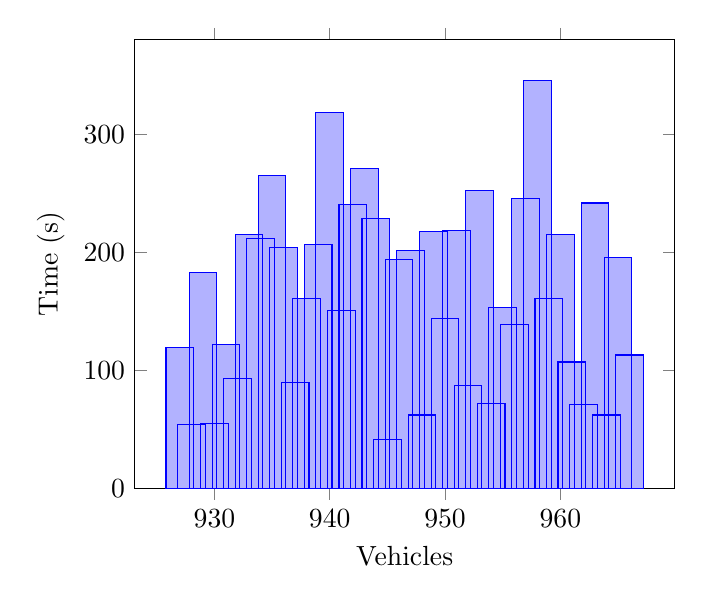
\begin{tikzpicture}
\begin{axis}[
legend style={anchor=west},
xlabel=Vehicles,
ylabel=Time (s),
ymin=0,
ybar,
]
\addplot coordinates {
(943, 271)
(944, 229)
(949, 218)
(942, 241)
(932, 93)
(950, 144)
(954, 72)
(958, 346)
(965, 196)
(964, 62)
(952, 87)
(946, 194)
(948, 62)
(928, 54)
(962, 71)
(947, 202)
(951, 219)
(956, 139)
(935, 265)
(966, 113)
(957, 246)
(930, 55)
(927, 119)
(933, 215)
(934, 212)
(931, 122)
(945, 41)
(959, 161)
(941, 151)
(936, 204)
(963, 242)
(953, 253)
(961, 107)
(940, 319)
(937, 90)
(938, 161)
(960, 215)
(955, 153)
(939, 207)
(929, 183)
};

\end{axis}
\end{tikzpicture}
\label{tik:time:0:13}
\caption{0 percent diving with GSC on route $13$}
\end{figure}
